\documentclass{article}
\usepackage[utf8]{inputenc}
\usepackage{natbib}
\usepackage{graphicx}
\usepackage[lofdepth,lotdepth]{subfig}

\title{Logic Gates and Flip-Flops}
\author{Oisín Peppard - 16323022}
\date{10/03/18}


\begin{document}

\maketitle

\section{Abstract}
In this experiment, we examine the functionality, and construct various elementary logic gates and flip-flops. We use a series of flip-flops to construct an asynchronous binary scaler that counts to 10 or 16. By constructing truth tables, we confirm functionality of AND, NAND, OR, NOR, XOR and XNOR gates and of a J-K Master Slave flip-flop.

\section{Basic Theory}
Logic gates are widely used devices, fundamental to most electronics. They perform logical functions on input signals such as counting or comparing them. In the apparatus for this experiment the input signals are 5V pulses. When an input pulse is present, we call this logical 1, an absence of signal is logical 0. This is the basis for Boolean algebra.

\begin{figure}[h!]
\centering
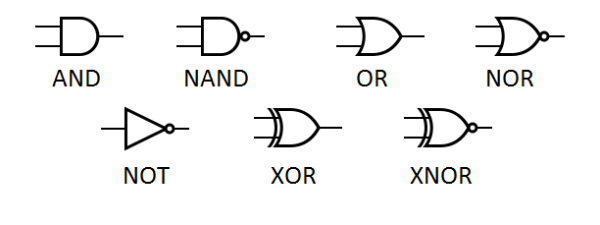
\includegraphics[width=\textwidth]{gates}
\caption{Symbols for various logic gates}
\label{fig:1}
\end{figure}

\subsection*{Types of logic gates examined}
\subsubsection*{The AND gate}
The AND gate gives a logical 1 if all inputs are 1, 0 otherwise.
\subsubsection*{The NAND gate}
This is the result of passing an AND through an inverter i.e. NOT gate. It gives a logical 0 if all inputs are 1 and 0 otherwise.
\subsubsection*{The OR gate}
This gives a logical 1 if any of its inputs are 1 and 0 if all inputs are 0.
\subsubsection*{The NOR gate}
This gives 0 if any inputs are 1 and 1 if all inputs are 0.
\subsubsection*{The NOT gate}
As is expected, this takes one input and changes from 0 to 1 or 1 to 0. Also called an inverter.
\subsubsection*{The XOR gate}
Short for exclusive or, similar to OR gate but gives a logical 0 if all inputs are 1.
\subsubsection*{The XNOR gate}
Exclusive NOR, gives logical 1 if all inputs are the same and 0 otherwise.

\vspace{5mm}
In this experiment, a positive TTL system is employed. We use an SN7400 2-input NAND gate, an SN7404 inverter, an SN7410 3-input NAND gate and an SN7476 J-K Flip-Flop. The other aforementioned gates are constructed by connecting these in various circuits.

\subsection*{The Clocked J-K Master Slave flip-flop}
This gate has four inputs; Ck(clock), J, K, Cr(clear) and Pr(set); and two outputs; Q and \=Q. The flip flop will be in a particular state and can be changed by the clock pulses but how it changes depends on the inputs at J and K. If both are 0, then the outputs do not change. If they are of opposite value, then the output will change only once. If they are both 1, then the output will change for each pulse.
 
\section{Experimental Method}
We use an apparatus consisting of input voltage sources controlled by switches, a series of logic gates on a board, with outputs to indicator LEDs. All operated on a 5V direct current.

\subsection*{NAND and AND gates}
We first verify the logic of our 3-input NAND gate. We use the SN7410 circuit with three integrated gates. The gate must first be powered by putting a 5V potential difference across it, and connecting it to earth. Connecting 5V pulse switches to the inputs, and the output to an indicator lamp, a truth table is constructed with the results of each input permutation. The effect of disconnecting one input is then observed and recorded. By passing the output of the NAND gate through an inverter, we construct an effective AND gate. Finally, we create an INHIBIT or VETO input, by passing one of the AND inputs through an inverter. See fig. 2 below. 

\begin{figure}[h]
    \centering
    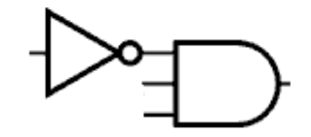
\includegraphics[scale = 0.35]{veto}
    \caption{COINCIDENCE-ANTICOINCIDENCE circuit}
    \label{fig:2}
\end{figure}

\subsection*{OR and NOR circuits}
In this part, we construct effective OR and NOR gates by combining the NAND and NOT gates in particular permutations. The circuit for an OR gate is shown below. The NOR gate is achieved by simply passing the output through an inverter. We check the logic of these gates and tabulate results.

\begin{figure}[h]
    \centering
    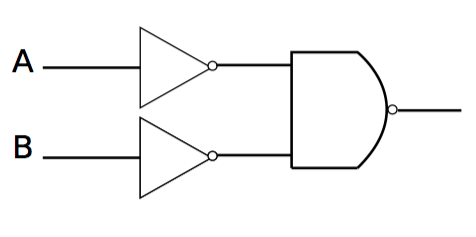
\includegraphics[scale = 0.35]{OR}
    \caption{OR circuit}
    \label{fig:3}
\end{figure}

\subsection*{XOR and XNOR circuits}
XOR and XNOR gates can similarly be constructed with a circuit. The set up is slightly more complex for these, and there are several possible setups. Three equivalent circuit diagrams for an effective exclusive OR gate is shown below. In each case, A and B are the two inputs, \=A and \=B are the two inputs passed through an inverter. We construct these circuits and verify their logic.

\begin{figure}[h]
\centering
\begin{minipage}[t]{0.23\textwidth}
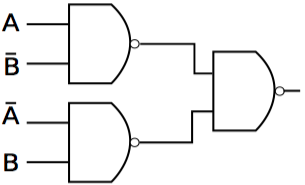
\includegraphics[width=\textwidth]{XOR1.png}
\caption*{XOR 1}
\end{minipage}
\begin{minipage}[t]{0.29\textwidth}
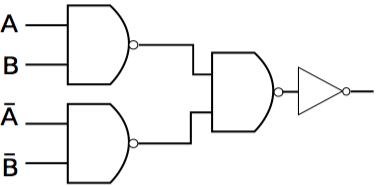
\includegraphics[width=\textwidth]{XOR2.png}
\caption*{XOR 2}
\end{minipage}
\begin{minipage}[t]{0.35\textwidth}
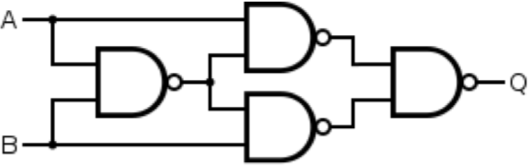
\includegraphics[width=\textwidth]{XOR3.png}
\caption*{XOR 3}
\end{minipage}
\caption{Equivalent XOR circuits}
\label{fig:4}   
\end{figure}

\subsection*{Flip-Flops}
A flip flop can be constructed from with four component logic gates, but we use one that is readily made. We connect first the J, K, and Clock inputs, and connect the outputs Q and \=Q to two indicator lamps. The results are recorded. The operation of the Clear and Preset inputs is then observed.

\begin{figure}[h]
    \centering
    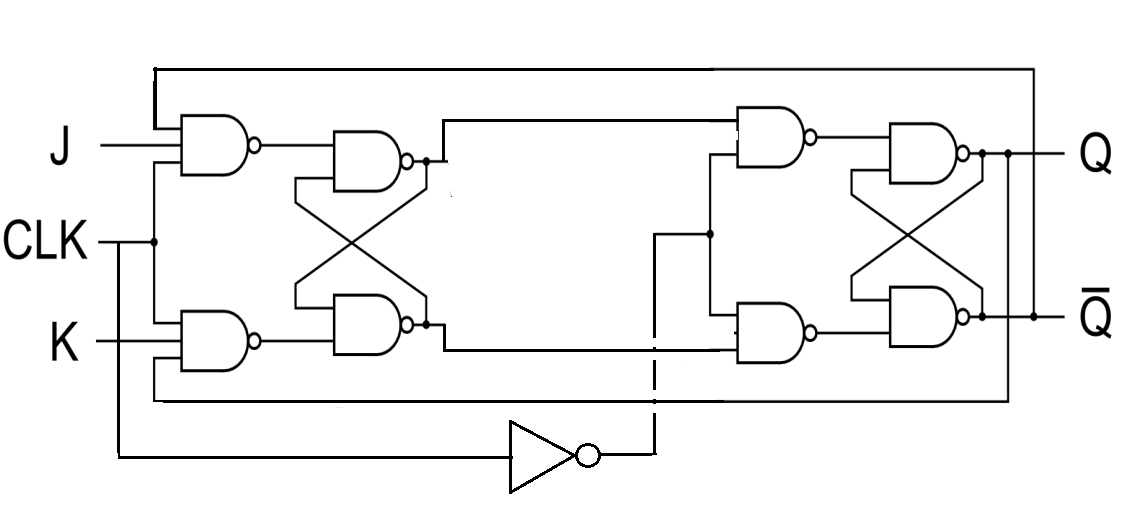
\includegraphics[scale = 0.3]{JK}
    \caption{Effective master-slave J-K flip-flop circuit}
    \label{fig:5}
\end{figure}
\begin{figure}[h!]
    \centering
    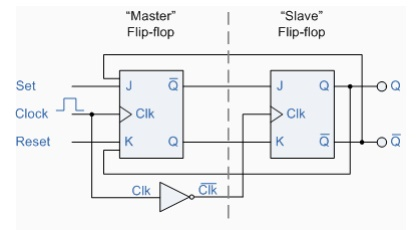
\includegraphics[scale = 0.6]{jkk}
    \caption{Master-Slave flip flop used in this experiment}
    \label{fig:6}
\end{figure}

\subsection*{Counters}
By connecting a series of flip-flop gates, a counter of scale 16 can be constructed. The circuit shown below (without the dotted lines) is constructed and the pattern recorded. The circuit is then extended along the dotted lines to produce an asynchronous counter of scale 10. 

\begin{figure}[h]
    \centering
    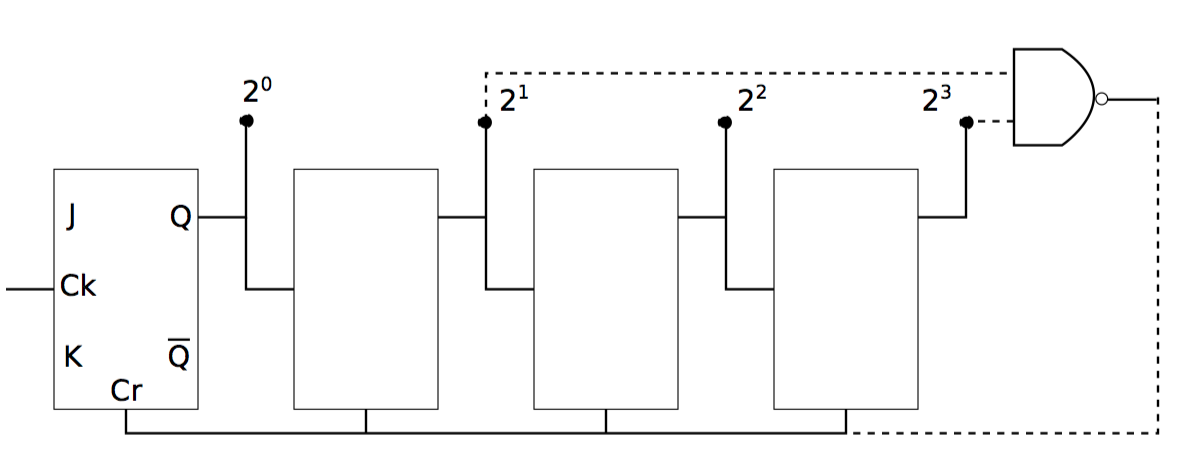
\includegraphics[width = \textwidth]{counter.png}
    \caption{Asynchronous counter of scale 10 or 16}
    \label{fig:7}
\end{figure}

\section{Results}
    \subsection*{NAND and AND gates}
    The truth tables are shown below for observed NAND and AND gate logic.\\
\vspace{2mm}    
\centering
\begin{table}[h]
\centering
\parbox{.45\linewidth}{
    \centering
    \begin{tabular}{c c c|c}
    A & B & C & Output\\
    \hline
    1&1&1&0\\
    1&0&1&1\\
    1&1&0&1\\
    0&1&1&1\\
    0&0&1&1\\
    1&0&0&1\\
    0&1&0&1\\
    0&0&0&1\\
    \end{tabular}
    \caption{NAND}
    \label{tab:1}
}   
\parbox{.45\linewidth}{
    \centering
    \begin{tabular}{c c c|c}
    A & B & C & Output\\
    \hline
    1&1&1&1\\
    1&0&1&0\\
    1&1&0&0\\
    0&1&1&0\\
    0&0&1&0\\
    1&0&0&0\\
    0&1&0&0\\
    0&0&0&0\\
    \end{tabular}
    \caption{AND}
    \label{tab:2}
}   
\end{table}

\vspace{2cm}
When input C was disconnected, the following logic was observed. 

\begin{table}[h]
    \centering
     \begin{tabular}{c c |c}
    A & B & Output\\
    \hline
    1&1&1\\
    1&0&0\\
    0&1&0\\
    0&0&0\\
    \end{tabular}
    \caption{AND with two inputs}
    \label{tab:6}
\end{table}

When input C was passed through an inverter, an INHIBIT/VETO switch was created and the following truth table was recorded.

\begin{table}[h]
    \centering
    \begin{tabular}{c c c|c}
    A & B & C & Output\\
    \hline
    1&1&1&0\\
    1&0&1&0\\
    1&1&0&1\\
    0&1&1&0\\
    0&0&1&0\\
    1&0&0&0\\
    0&1&0&0\\
    0&0&0&0\\
    \end{tabular}
    \caption{VETO switch AND gate}
    \label{tab:7}
\end{table}


\vspace{2cm}    

\subsection*{OR and NOR circuits}
The truth tables are shown below for observed OR and NOR gates.
\begin{table}[h]
\centering
\parbox{.45\linewidth}{
    \centering
    \begin{tabular}{c c | c}
    A & B & Output\\
    \hline
    1&1&1\\
    1&0&1\\
    0&1&1\\
    0&0&1\\
    \end{tabular}
    \caption{OR}
    \label{tab:3}
}   
\parbox{.45\linewidth}{
    \centering
    \begin{tabular}{c c |c}
    A & B & Output\\
    \hline
    1&1&0\\
    1&0&0\\
    0&1&0\\
    0&0&1\\
    \end{tabular}
    \caption{NOR}
    \label{tab:4}
}   
\end{table}

\vspace{3cm}
\subsection*{XOR and XNOR circuits}
Results for XOR and XNOR logic.
\begin{table}[h]
\centering
\parbox{.45\linewidth}{
    \centering
    \begin{tabular}{c c | c}
    A & B & Output\\
    \hline
    1&1&0\\
    1&0&1\\
    0&1&1\\
    0&0&0\\
    \end{tabular}
    \caption{XOR}
    \label{tab:8}
}
\parbox{.45\linewidth}{
    \centering
    \begin{tabular}{c c | c}
    A & B & Output\\
    \hline
    1&1&1\\
    1&0&0\\
    0&1&0\\
    0&0&1\\
    \end{tabular}
    \caption{XNOR}
    \label{tab:5}
}
\end{table}

\subsection*{Flip-Flops}
\subsubsection*{J and K logic}
\begin{itemize}
    \item When J = 1, K = 0, the outputs are Q = 1, \=Q = 0 always.
    \item When J = 0, K = 1
        \begin{itemize}
            \item If Q, \=Q start at 1, 0 respectively, the output changes to 0, 1 when a clock pulse is received. 
            \item If Q, \=Q start at 0, 1 respectively, the output remains unchanged when a clock pulse is received.
        \end{itemize}
    \item When J = 1, K = 1, Q = 0, \=Q = 1 until a clock signal is received each signal is inverted. The outputs continue to invert on each clock pulse resulting in an alternating on/off pattern of Q and \=Q.
    \item When J = 0, K = 0, the clock had no effect on the output states.
    \item When J and K were disconnected, the same alternating result as J = 1, K = 1 was observed.
\end{itemize}
\subsubsection*{Clear and Preset}
It was found that the clear function would return Q to 1, \=Q = 0, regardless of the state of J or K, thus 'clearing' the flip-flop state. Similarly, the preset function set Q = 0, \=Q = 1, effectively 'presetting' the condition.

\vspace{3cm}
\subsection*{Counters}
When the flip-flop gates are set up in the layout described above, the following results were recorded for an asynchronous timer of scale 16.
\begin{table}[h!]
    \centering
    \begin{tabular}{c|c c c c}
         Pulse & 2^0 & 2^1 & 2^2 & 2^3 \\
         \hline
         0& 0& 0& 0& 0\\
         1& 1& 0& 0& 0\\
         2& 0& 1& 0& 0\\
         3& 1& 1& 0& 0\\
         4& 0& 0& 1& 0\\
         5& 1& 0& 1& 0\\
         6& 0& 1& 1& 0\\
         7& 1& 1& 1& 0\\
         8& 0& 0& 0& 1\\
         9& 1& 0& 0& 1\\
         10& 0& 1& 0& 1\\
         11& 1& 1& 0& 1\\
         12& 0& 0& 1& 1\\
         13& 1& 0& 1& 1\\
         14& 0& 1& 1& 1\\
         15& 1& 1& 1& 1\\
         16& 0& 0& 0& 0\\
    \end{tabular}
    \caption{Scale 16}
    \label{tab:9}
\end{table}

\begin{table}[h!]
    \centering
    \begin{tabular}{c|c c c c}
         Pulse & 2^0 & 2^1 & 2^2 & 2^3 \\
         \hline
         0& 0& 0& 0& 0\\
         1& 1& 0& 0& 0\\
         2& 0& 1& 0& 0\\
         3& 1& 1& 0& 0\\
         4& 0& 0& 1& 0\\
         5& 1& 0& 1& 0\\
         6& 0& 1& 1& 0\\
         7& 1& 1& 1& 0\\
         8& 0& 0& 0& 1\\
         9& 1& 0& 0& 1\\
         10& 0& 1& 0& 1\\
    \end{tabular}
    \caption{Scale 10}
    \label{tab:9}
\end{table}

Counters of other scales can be achieved by connecting the required inputs to the NAND gate which would produce an output when the number is reached by clearing the flip flops.

\section{Conclusions and discussion}

It was found that the NAND and AND logic works as expected, removing one input from a 3-input AND gate leaves an effective 2-input AND gate.
The VETO input effectively creates an switch that will prevent any signal passing through while switched on, thus inhibiting the pulse.It is essentially a 2-input AND gate with an extra event; a switch that must be off. This is called a COINCIDENCE-ANTICOINCIDENCE circuit.
\vspace{3mm}
Once circuits are constructed, it is found that OR and NOR gates function as expected and their logic is verified.
\vspace{3mm}
Exclusive OR gate works to provide a pulse if and only if exactly one of its two inputs is logical 1. XNOR gives a pulse if both inputs are the same. This can effectively be used as a comparator.
\vspace{3mm}
The behaviour of a flip-flop allows for creation of timers.
\vspace{3mm}
The counters of scales 16 and 10 work effectively to count to these numbers in binary, with each indicator light representing a power of 2.

\end{document}

